\documentclass[twocolumn]{autart}

%\input{doiCmd}
%\RequirePackage{doi}
\usepackage[
	pdftitle={Sphere 7 Data: LOUD and FAIR Data for the Research Community},
	pdfsubject={Sphere 7 Data: LOUD and FAIR Data for the Research Community},
	pdfauthor={Florian Thiery},
	pdfkeywords={Linked Data, Linked Open Data, Five Star Data, FAIR Data, Semantic Web}
]{hyperref}

\usepackage{graphicx}          % Include this line if your 
                               % document contains figures,
%\usepackage[dvips]{epsfig}    % or this line, depending on which
                               % you prefer.
\usepackage{verbatimbox}

\usepackage[german, english]{babel} 

\usepackage{mnsymbol}

\usepackage{url}

\usepackage{xcolor}

\begin{document}\selectlanguage{english}

\begin{frontmatter}
%\runtitle{Insert a suggested running title}  % Running title for regular 
                                              % papers but only if the title  
                                              % is over 5 words. Running title 
                                              % is not shown in output.

\title{Sphere 7 Data: \protect\\ LOUD and FAIR Data for the Research Community}
                                               

\author[FT]{Florian Thiery}

\address[FT]{rse@fthiery.de - ORCID: 0000-0002-3246-3531 \protect\\ Research Software Engineer, R\"omisch-Germanisches Zentralmuseum, Mainz, Germany}                                         

          
\begin{keyword}                             
Linked Data; Linked Open Data; Five Star Data; FAIR Data; Semantic Web. 
\end{keyword}

\begin{abstract}                         

The world of data modelling, publishing and sharing has changed rapidly in the last years. Starting from the invention of the World Wide Web in 1989 by Sir Tim Berners-Lee this Web is on an evolution to the so called Web 4.0. Before we will reach that we have to ‘fill’ the Semantic Web as part of the Web 3.0 with resources and research content. Therefore the 5 star open data principles, the Linked Open Data principles, the 5 star LOUD principles and the FAIR principles are necessary. I will merge all of that principles in the so called \textbf{Sphere 7 Data principles}, described in this paper.

\end{abstract}

\end{frontmatter}

\section{Introduction}

In some old maps (Fig.~\ref{map}) of the ancient world the phrase \textbf{'Hic sunt dracones'} (engl. \textit{Here be Dragons})\cite{wuttke_here_2019-1} is used to describe an area, that is unknown to the map creator. As Ulrike Wuttke\footnote{\url{https://twitter.com/uwuttke}} mentioned, this is quite appropriate to summarise the ambivalence of humanists towards data and these 'fancy' new concepts\cite{wuttke_here_2019} in this digital new thing, called the World Wide Web and the Internet.

\begin{figure}[!htb]
\begin{center}
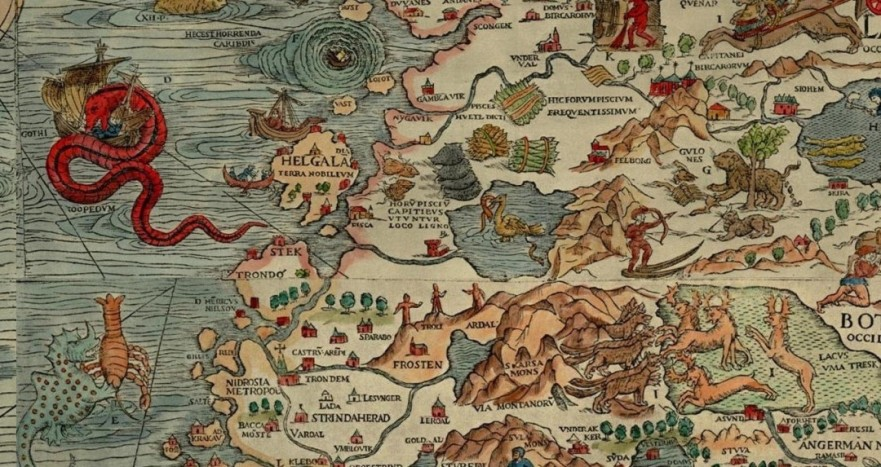
\includegraphics[width=8cm]{Beyond-This-here-be-no-dragons-blog-copy-881x467.jpg}
\caption{Nature and Science, https://t1p.de/wmtz}
\label{map}
\end{center}
\end{figure}

The WWW give researchers a new possibility to share there special research data with other (non subject-specific) communities, link them to other available data on the internet and enable the creation of new unknown knowledge. Maybe a good technique to fight against the data dragons (Fig.~\ref{datadragon}) in research!

\begin{figure}[!htb]
\begin{center}

\includegraphics[width=6cm]{datadragon.png}
\caption{Fight against the data dragons}
\label{datadragon}
\end{center}
\end{figure}

Here the techniques of the Semantic Web\cite{BernersLee2001TheSW} as part of the Web 3.0 comes into play. Using the idea of Open Data in mind, combined with RDF, several semantically described links, usable interfaces and applications for data, as well as FAIR data principles, will be possible to create a huge research data cloud (Fig.~\ref{ldc}).

\begin{figure}[!htb]
\begin{center}
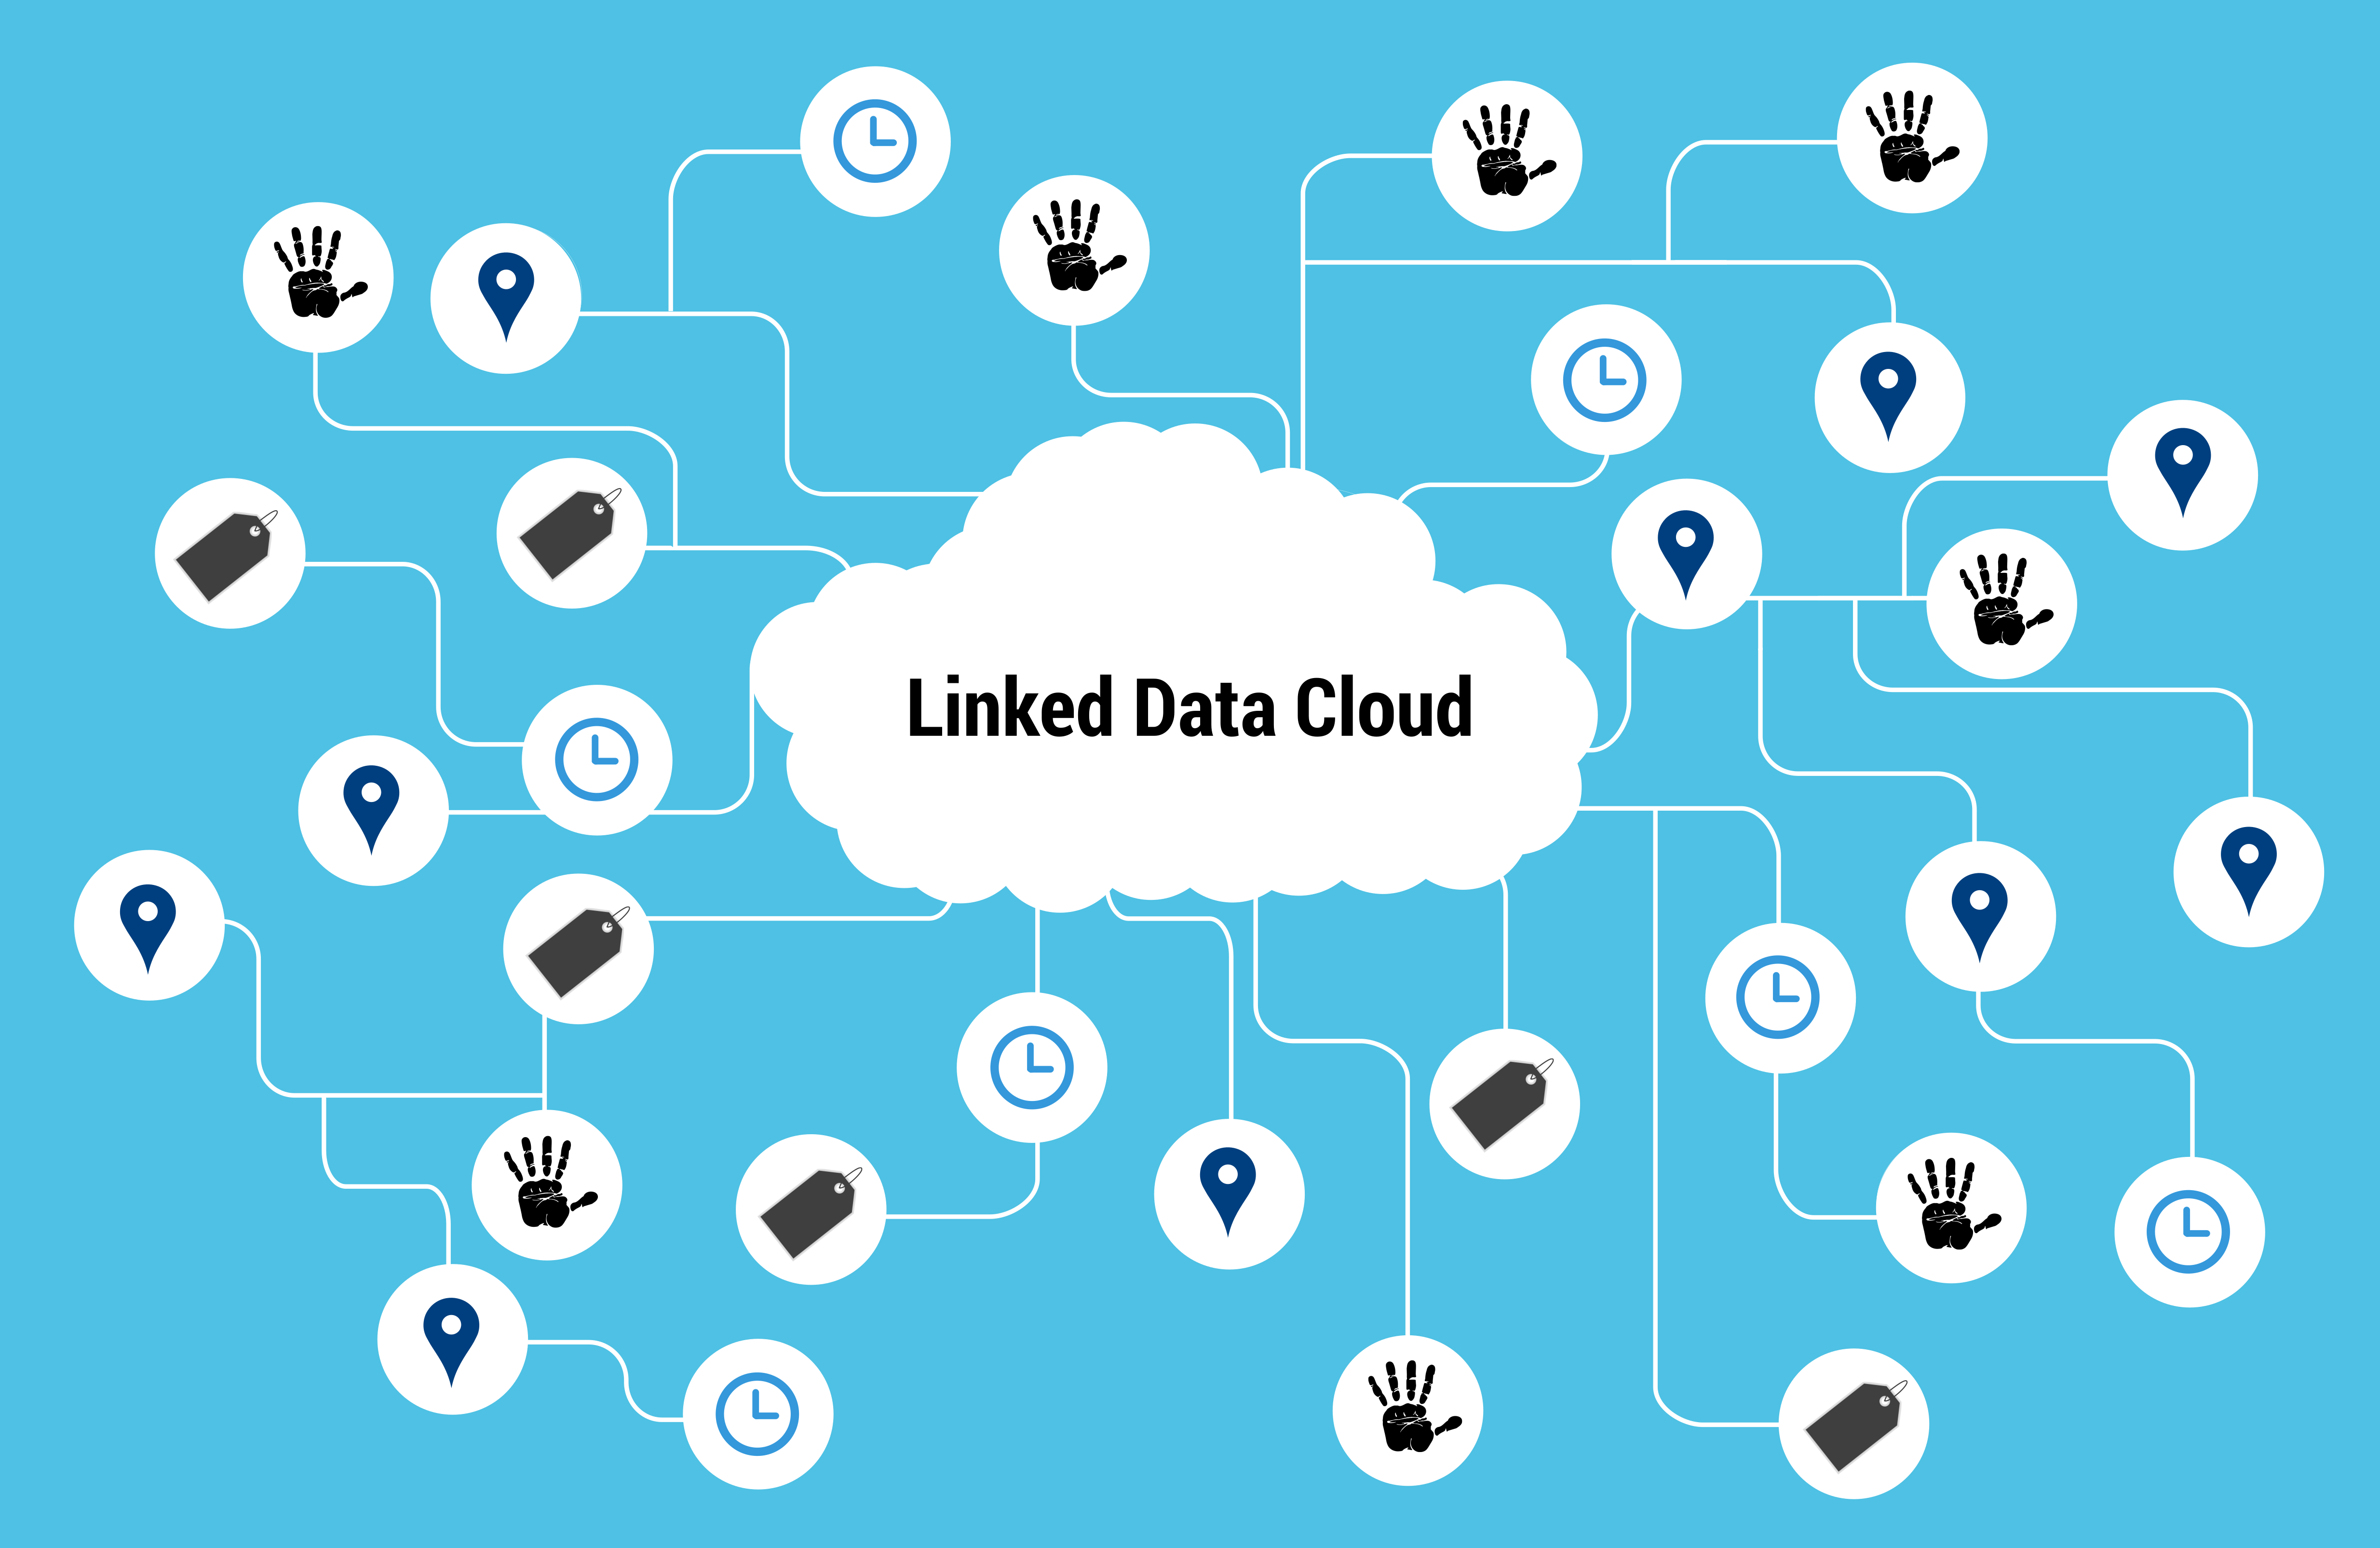
\includegraphics[width=8cm]{ldc.png}
\caption{Linked Data Cloud Scheme, Florian Thiery [CC BY 4.0]}
\label{ldc}
\end{center}
\end{figure}

The aim should be the creation of a huge data graph (Fig.~\ref{graph}) as part of the \textit{Linked Open Data Cloud}\footnote{\url{http://lod-cloud.net}} or \textit{Giant Global Graph} (GGG) using the principles described in the next sections: (1) the five stars of Open Data, (2) the four Linked Data principles, (3) the five stars of Linked Open Usable Data (LOUD) and (4) the 15 FAIR data principles to end up in a model, what I will call the \textbf{Sphere 7 Data} principles.

\begin{figure}[!htb]
\begin{center}
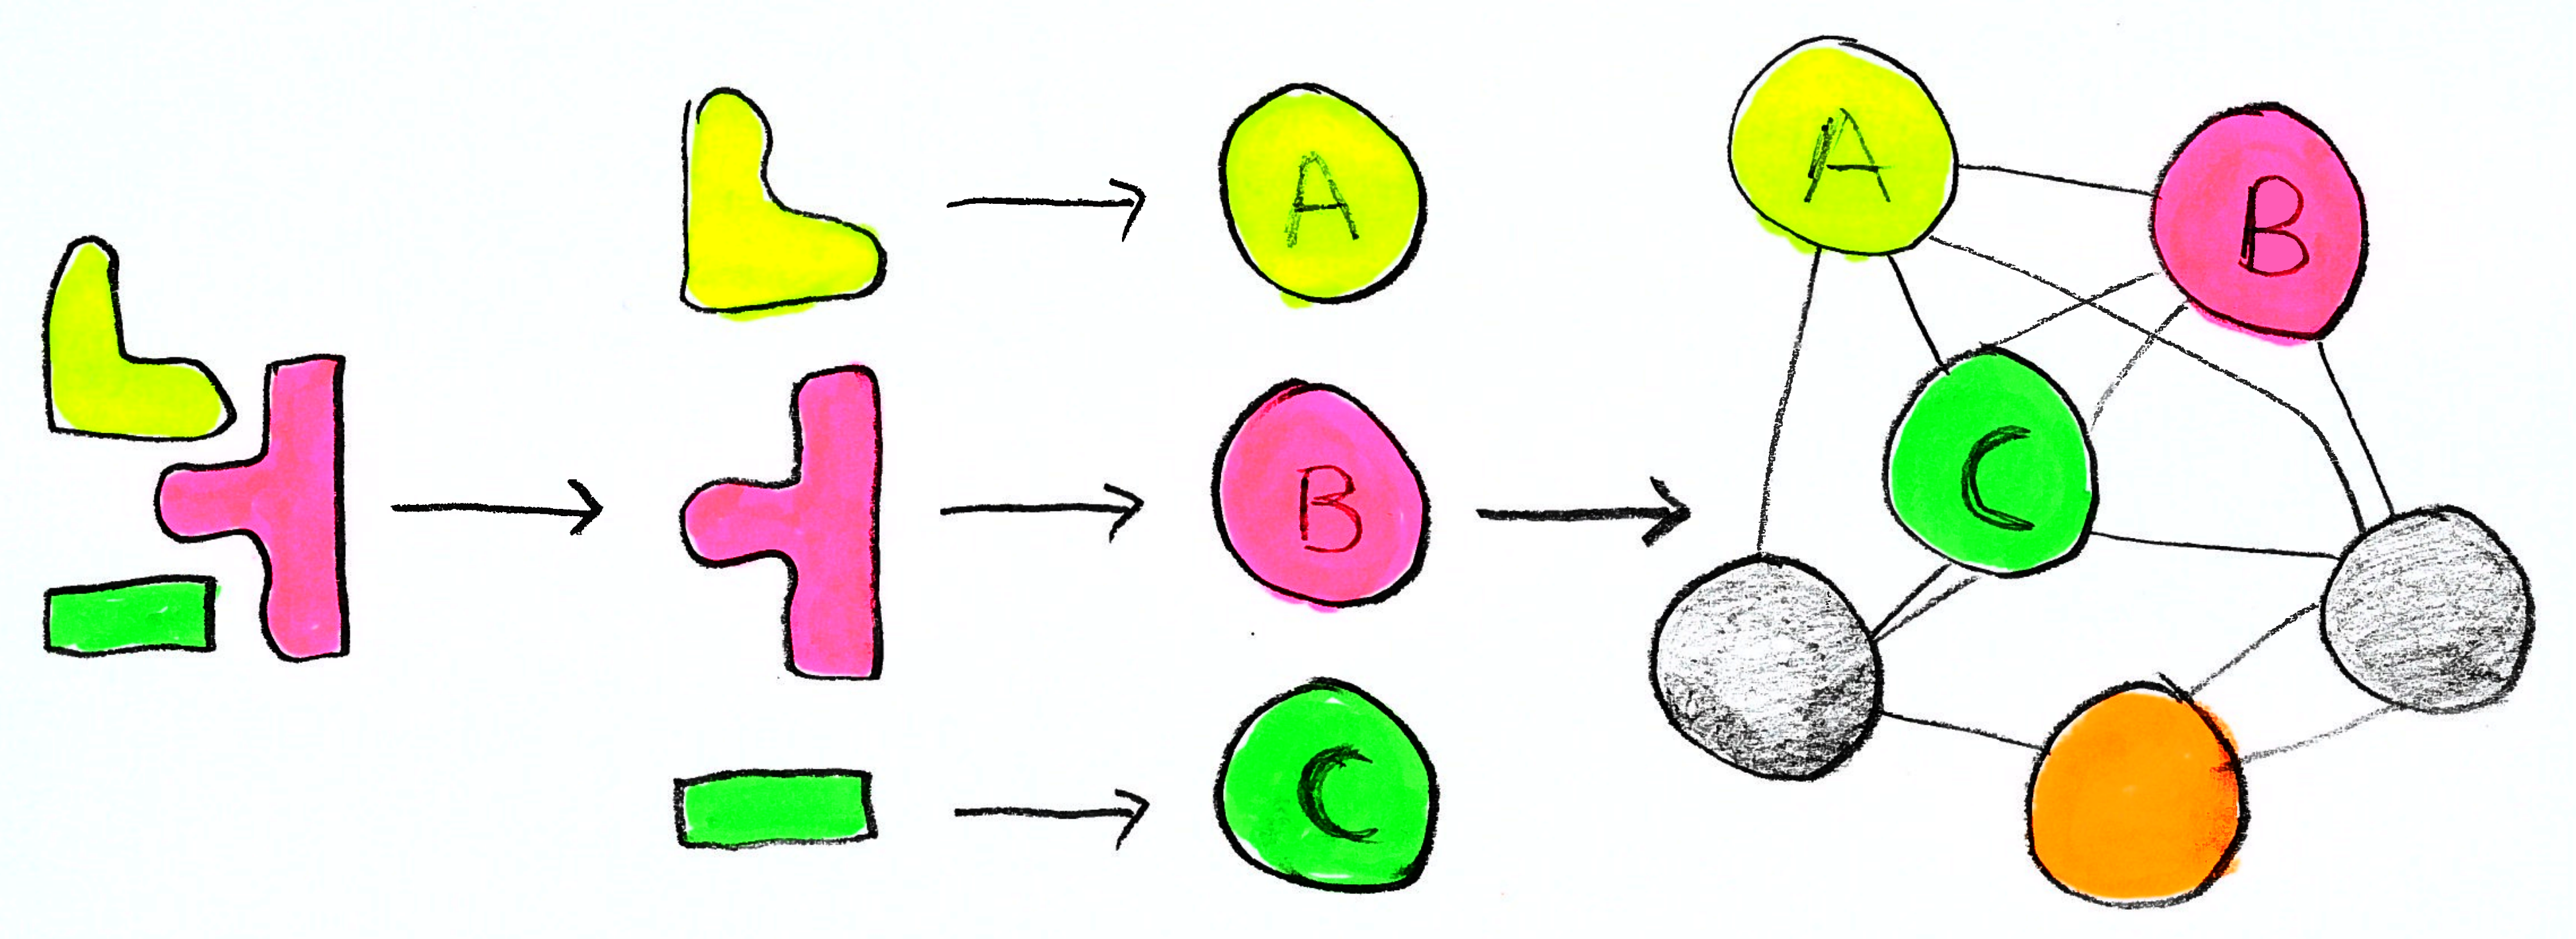
\includegraphics[width=8cm]{Graph_From_Data_Pieces.png}
\caption{Graph From Data Pieces, Florian Thiery [CC BY 4.0]}
\label{graph}
\end{center}
\end{figure}

\section{Linked Data Principles}

Referring to Tim Berners-Lee\footnote{\url{https://twitter.com/timberners_lee}} \frqq\textit{The Web does not just connect machines, it connects people.}\flqq it is the same with data and research data:

\begin{verse}
	\textbf{The Web does not just connect machines, it connects data and thus knowledge of people!}
\end{verse}

But to do this, some technique and 'standards' had to be build. In his first publication on Linked Data, Tim Berners-Lee wrote:

\begin{quotation}
	\frqq\textit{The Semantic Web isn't just about putting data on the web. It is about making links, so that a person or machine can explore the web of data. With linked data, when you have some of it, you can find other, related, data.}\flqq\cite{berners-lee_linked_2006}
\end{quotation}

\begin{quotation}
	\frqq\textit{Like the web of hypertext, the web of data is constructed with documents on the web. However, unlike the web of hypertext, where links are relationships anchors in hypertext documents written in HTML, for data they links between arbitrary things described by RDF, the URIs identify any kind of object or concept. But for HTML or RDF, the same expectations apply to make the web grow.}\flqq\cite{berners-lee_linked_2006}
\end{quotation}

Tim Berners-Lee ended up in defining \frqq\textit{imperfect but published}\flqq\cite{berners-lee_linked_2006} four simple rules for Linked Data (on 2006-07-27), the so called Linked Data principles\cite{berners-lee_linked_2006}, illustrated in Fig.~\ref{ld}:

\begin{quotation}
\begin{enumerate}
	\item Use URIs as names for things
	\item Use HTTP URIs so that people can look up those names.
	\item When someone looks up a URI, provide useful information, using the standards (RDF*, SPARQL)
	\item Include links to other URIs. so that they can discover more things.
\end{enumerate}
\end{quotation}

\begin{figure}[!htb]
\begin{center}
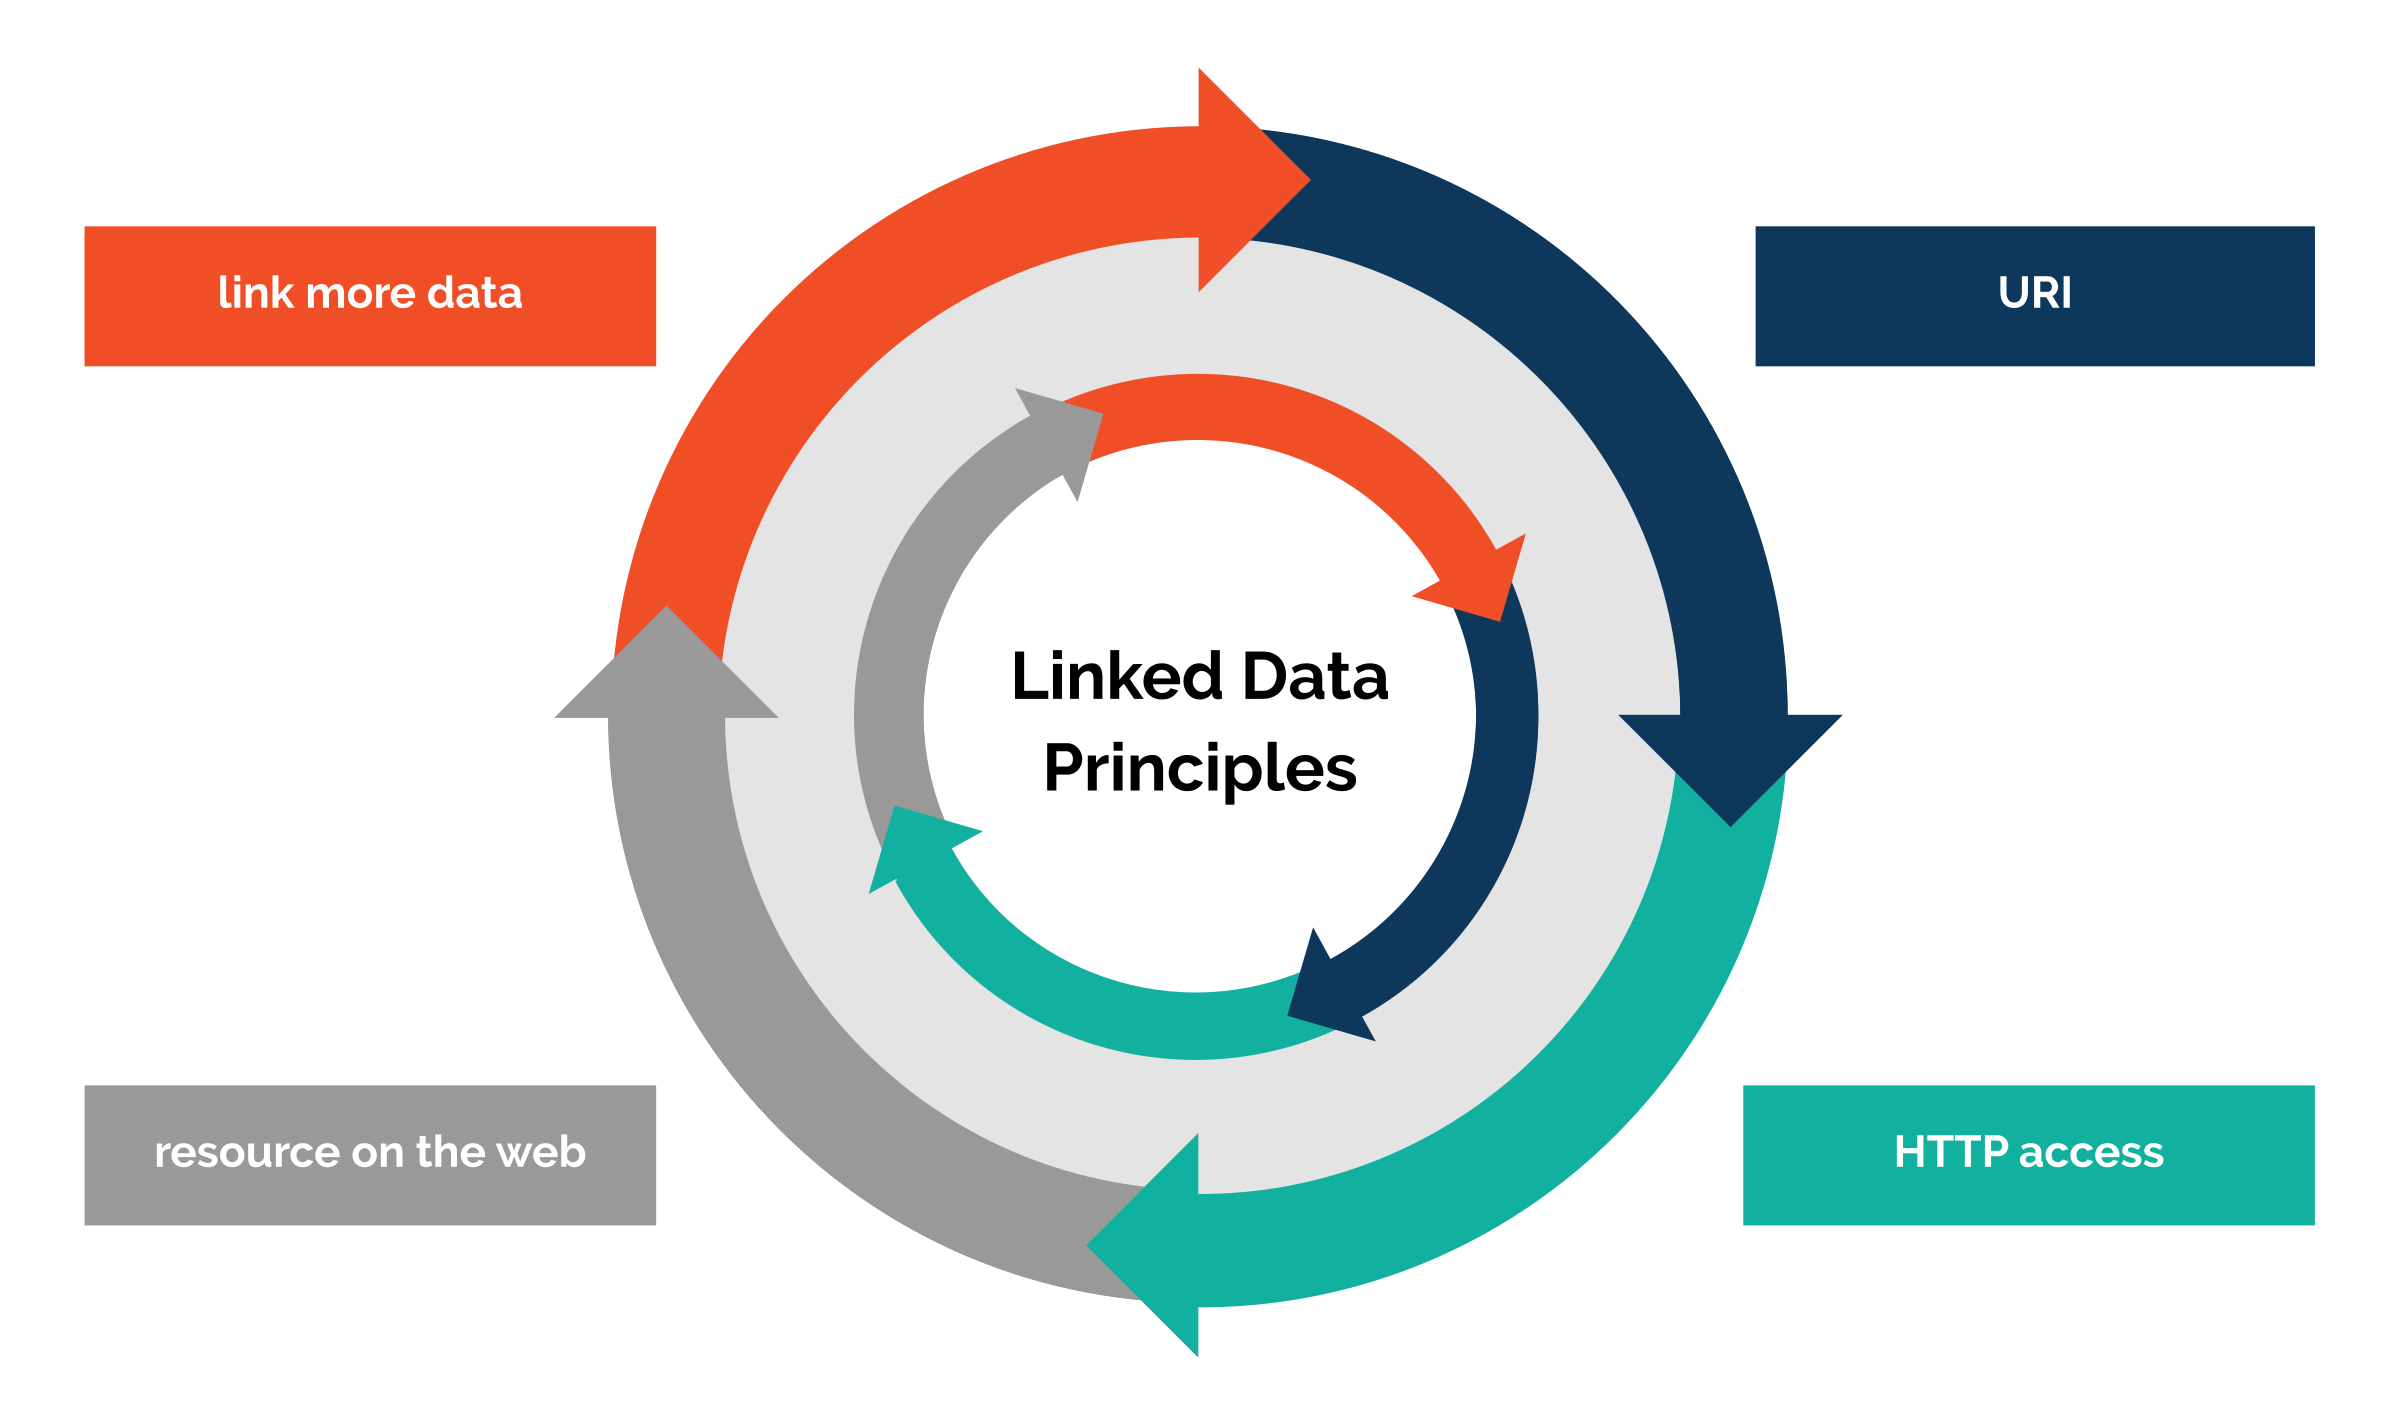
\includegraphics[width=8cm]{Linked_Data_Principles.png}
\caption{Linked Data Principles, Florian Thiery [CC BY 4.0]}
\label{ld}
\end{center}
\end{figure}

\section{Five stars of Open Data}

In an ideal world, research data and all other kind of data are published and available for everyone, from every place on this planet. To reach this, data must be published OPEN.

The idea and most important facts of Open Data\footnote{\url{https://opendefinition.org/od/2.1/en/}} can be summarised \footnote{\url{http://opendatahandbook.org/guide/en/what-is-open-data/}} as follows: (1) availability and access, (2) re-use and redistribution and (3) universal participation. So it is all about interoperability!

This idea in mind, Sir Tim Berners-Lee started to ask in 2010: 'Is your Linked Open Data 5 star?':

\begin{quotation}
	\frqq\textit{This year, in order to encourage people -- especially government data owners -- along the road to good linked data, I have developped[sic!] [a] star rating system. [...] Linked \textit{Open} Data (LOD) is Linked Data which is released under an open licence, which does not impede its reuse for free. [...]. Linked Data does not of course in general have to be open -- there is a lot of important use of lnked[sic!] data internally, and for personal and group-wide data. You can have 5-star Linked Data without it being open. However, if it claims to be Linked Open Data then it does have to be open, to get any star at all.}\flqq\cite{berners-lee_linked_2006}
\end{quotation}

The five star rating system for 5 Star Open Data is shown in Fig.~\ref{5sd}. The five star data website\cite{hausenblas_5-sterne_2015} introduces in the principles as follows:

\begin{itemize}
	\item $\medstar$ make your stuff available on the Web (whatever format) under an open license
	\item $\medstar\medstar$ make it available as structured data (e.g., Excel instead of image scan of a table)
	\item $\medstar\medstar\medstar$ make it available in a non-proprietary open format (e.g., CSV instead of Excel)
	\item $\medstar\medstar\medstar\medstar$ use URIs to denote things, so that people can point at your stuff
	\item $\medstar\medstar\medstar\medstar\medstar$ link your data to other data to provide context
\end{itemize}

\begin{figure}[!htb]
\begin{center}
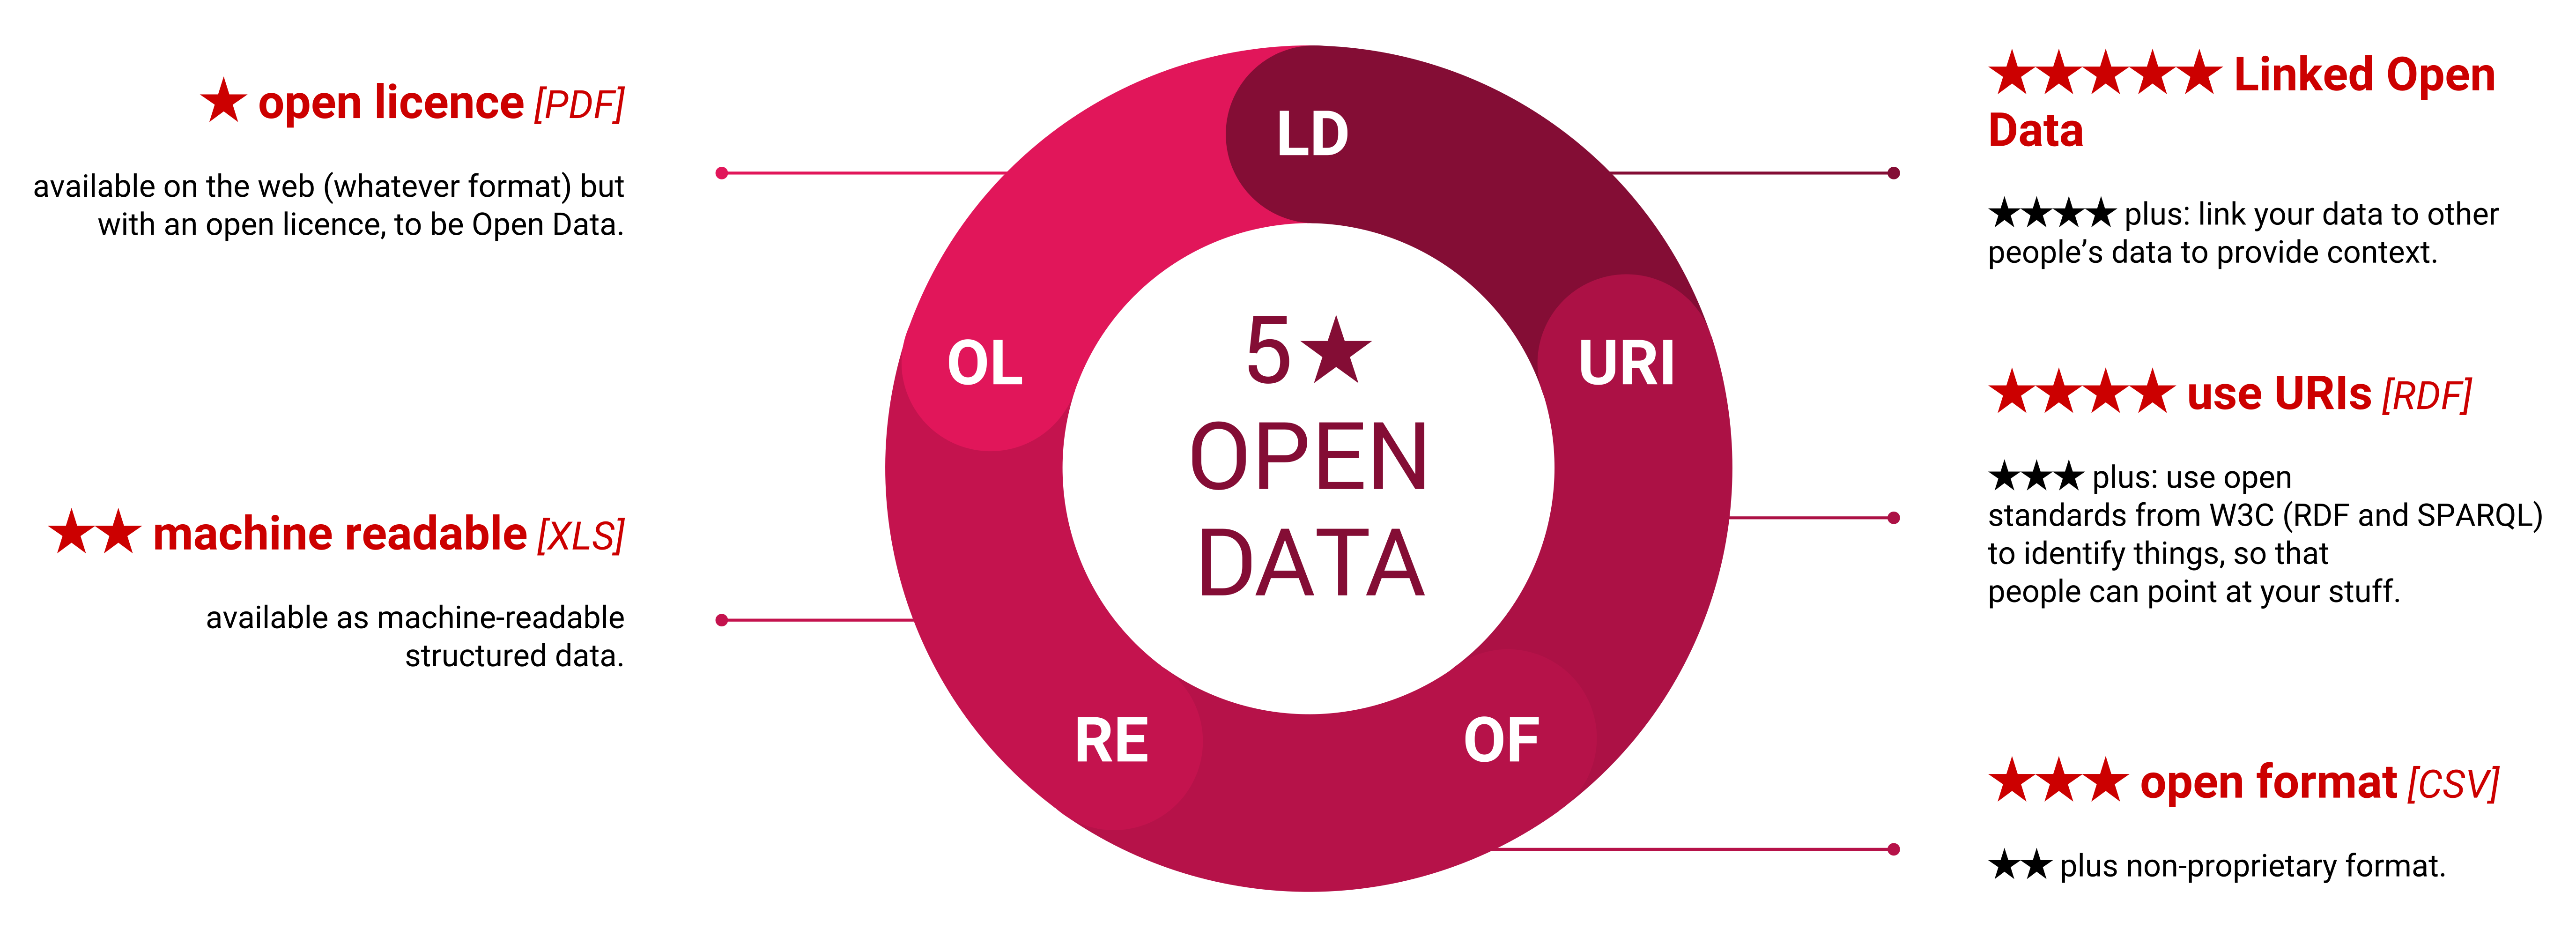
\includegraphics[width=8cm]{5_Star_Open_Data.png}
\caption{5 Star Open Data, Florian Thiery [CC BY 4.0]}
\label{5sd}
\end{center}
\end{figure}

\section{Five stars of LOUD}

On top of the before mentioned 5 Star Linked Open Data modelling summit, the (semantic) Information Architect at The Getty Trust, Rob Sanderson,\footnote{\url{https://twitter.com/azaroth42}} shouted his further A-B-C-D-E ideas out LOUD at his \textit{EuropeanaTech} keynote\cite{sanderson_shout_2018} in 2018\footnote{\url{https://youtu.be/r4afi8mGVAY}}.

\begin{quotation}
	\frqq\textit{Linked Open Data, with its five stars of excellence, changed the way that we publish data on the web. It gave us a short and very practical checklist that we could use to go from thinking about semantics to publishing actual data. It promotes openness as a necessity for reuse. It promotes standards as a necessity for reuse. It promotes linking between systems as a necessity for reuse. But it comes exclusively from a publishing perspective, and does not make any recommendations about how to publish data in a way that is usable by potential consumers. In the intervening time, the web community has recognized that we need 5 more stars for data consumption. If our data isn't used, then no value is gained from the resources that were invested in its creation, publication, maintenance and improvement. If we want our data to be used, then it needs to be \textbf{usable}: Linked Open Usable Data.}\flqq\cite{sanderson_loud_2018}
\end{quotation}

\begin{quotation}
	\frqq\textit{Meaning that Usability is dependent upon the audience. And the Audience for Data is Developers. The user interface for developers is the API, and the API for LOD is based on the ontology. Ontologies are design primarily for semantic or theoretical correctness, which is the least practical concern. Instead, we need to manage the complexities between completeness of expression, and usability of the resulting data constructs. JSON-LD allows for some mapping of ontological constructs into JSON, the lingua-franca of modern developers and is a cornerstone technology of LOUD. Five further stars, or design principles, govern usability.}\flqq\cite{sanderson_loud_2018}
\end{quotation}

The five further stars to produce LOUD instead of LOD will be \cite{sanderson_loud_2018}:

1. The right Abstraction for the audience

\textit{As we all know \frqq developers do not need the same level of access to data as a ontologist. Here, some use cases and requirements should drive the interoperability layer between systems, not ontologies. \flqq}

2. Few Barriers to entry

For developers it should \frqq be easy to get started with the LOD and build something \flqq immediately. \frqq If it takes a long time to understand the model, ontology, sparql query syntax and so forth, then developers will look for easier targets. Conversely, if it is easy to start and incrementally improve, more [and more] people will use the data. \flqq

3. Comprehensible by introspection

\textit{Published and shared \frqq data should be understandable by looking at it, rather than requiring the developer to read the ontology and vocabularies. \flqq By \frqq using [e.g.] JSON-LD[, it] lets us to talk to the developer in their language, that they already understand. \flqq}

4. Documentation with working examples

\textit{Data have to be comprehensible and well documented. \frqq You can never \flqq get all the 'hidden assumptions' and \frqq all of the rules for the data. Documentation clarifies the patterns that the developer can expect to encounter, such that they can implement robustly. Example use cases allow contextualization for when the pattern will be encountered, and working examples let you drop the data into the system to see if it implements that pattern correctly. \flqq}

5. Few Exceptions, many consistent patterns

\textit{\frqq Every exception that you have in an API [or ontology] is another rule that the developer needs to learn in order to use the system. Every exception is jarring, and requires additional code to manage. While not everything is homogenous, a set of patterns that manage exceptions well is better than many custom fields. \flqq}

Check Fig.~\ref{loud} so see quickly how your LOD can be LOUD.

\begin{figure}[!htb]
\begin{center}
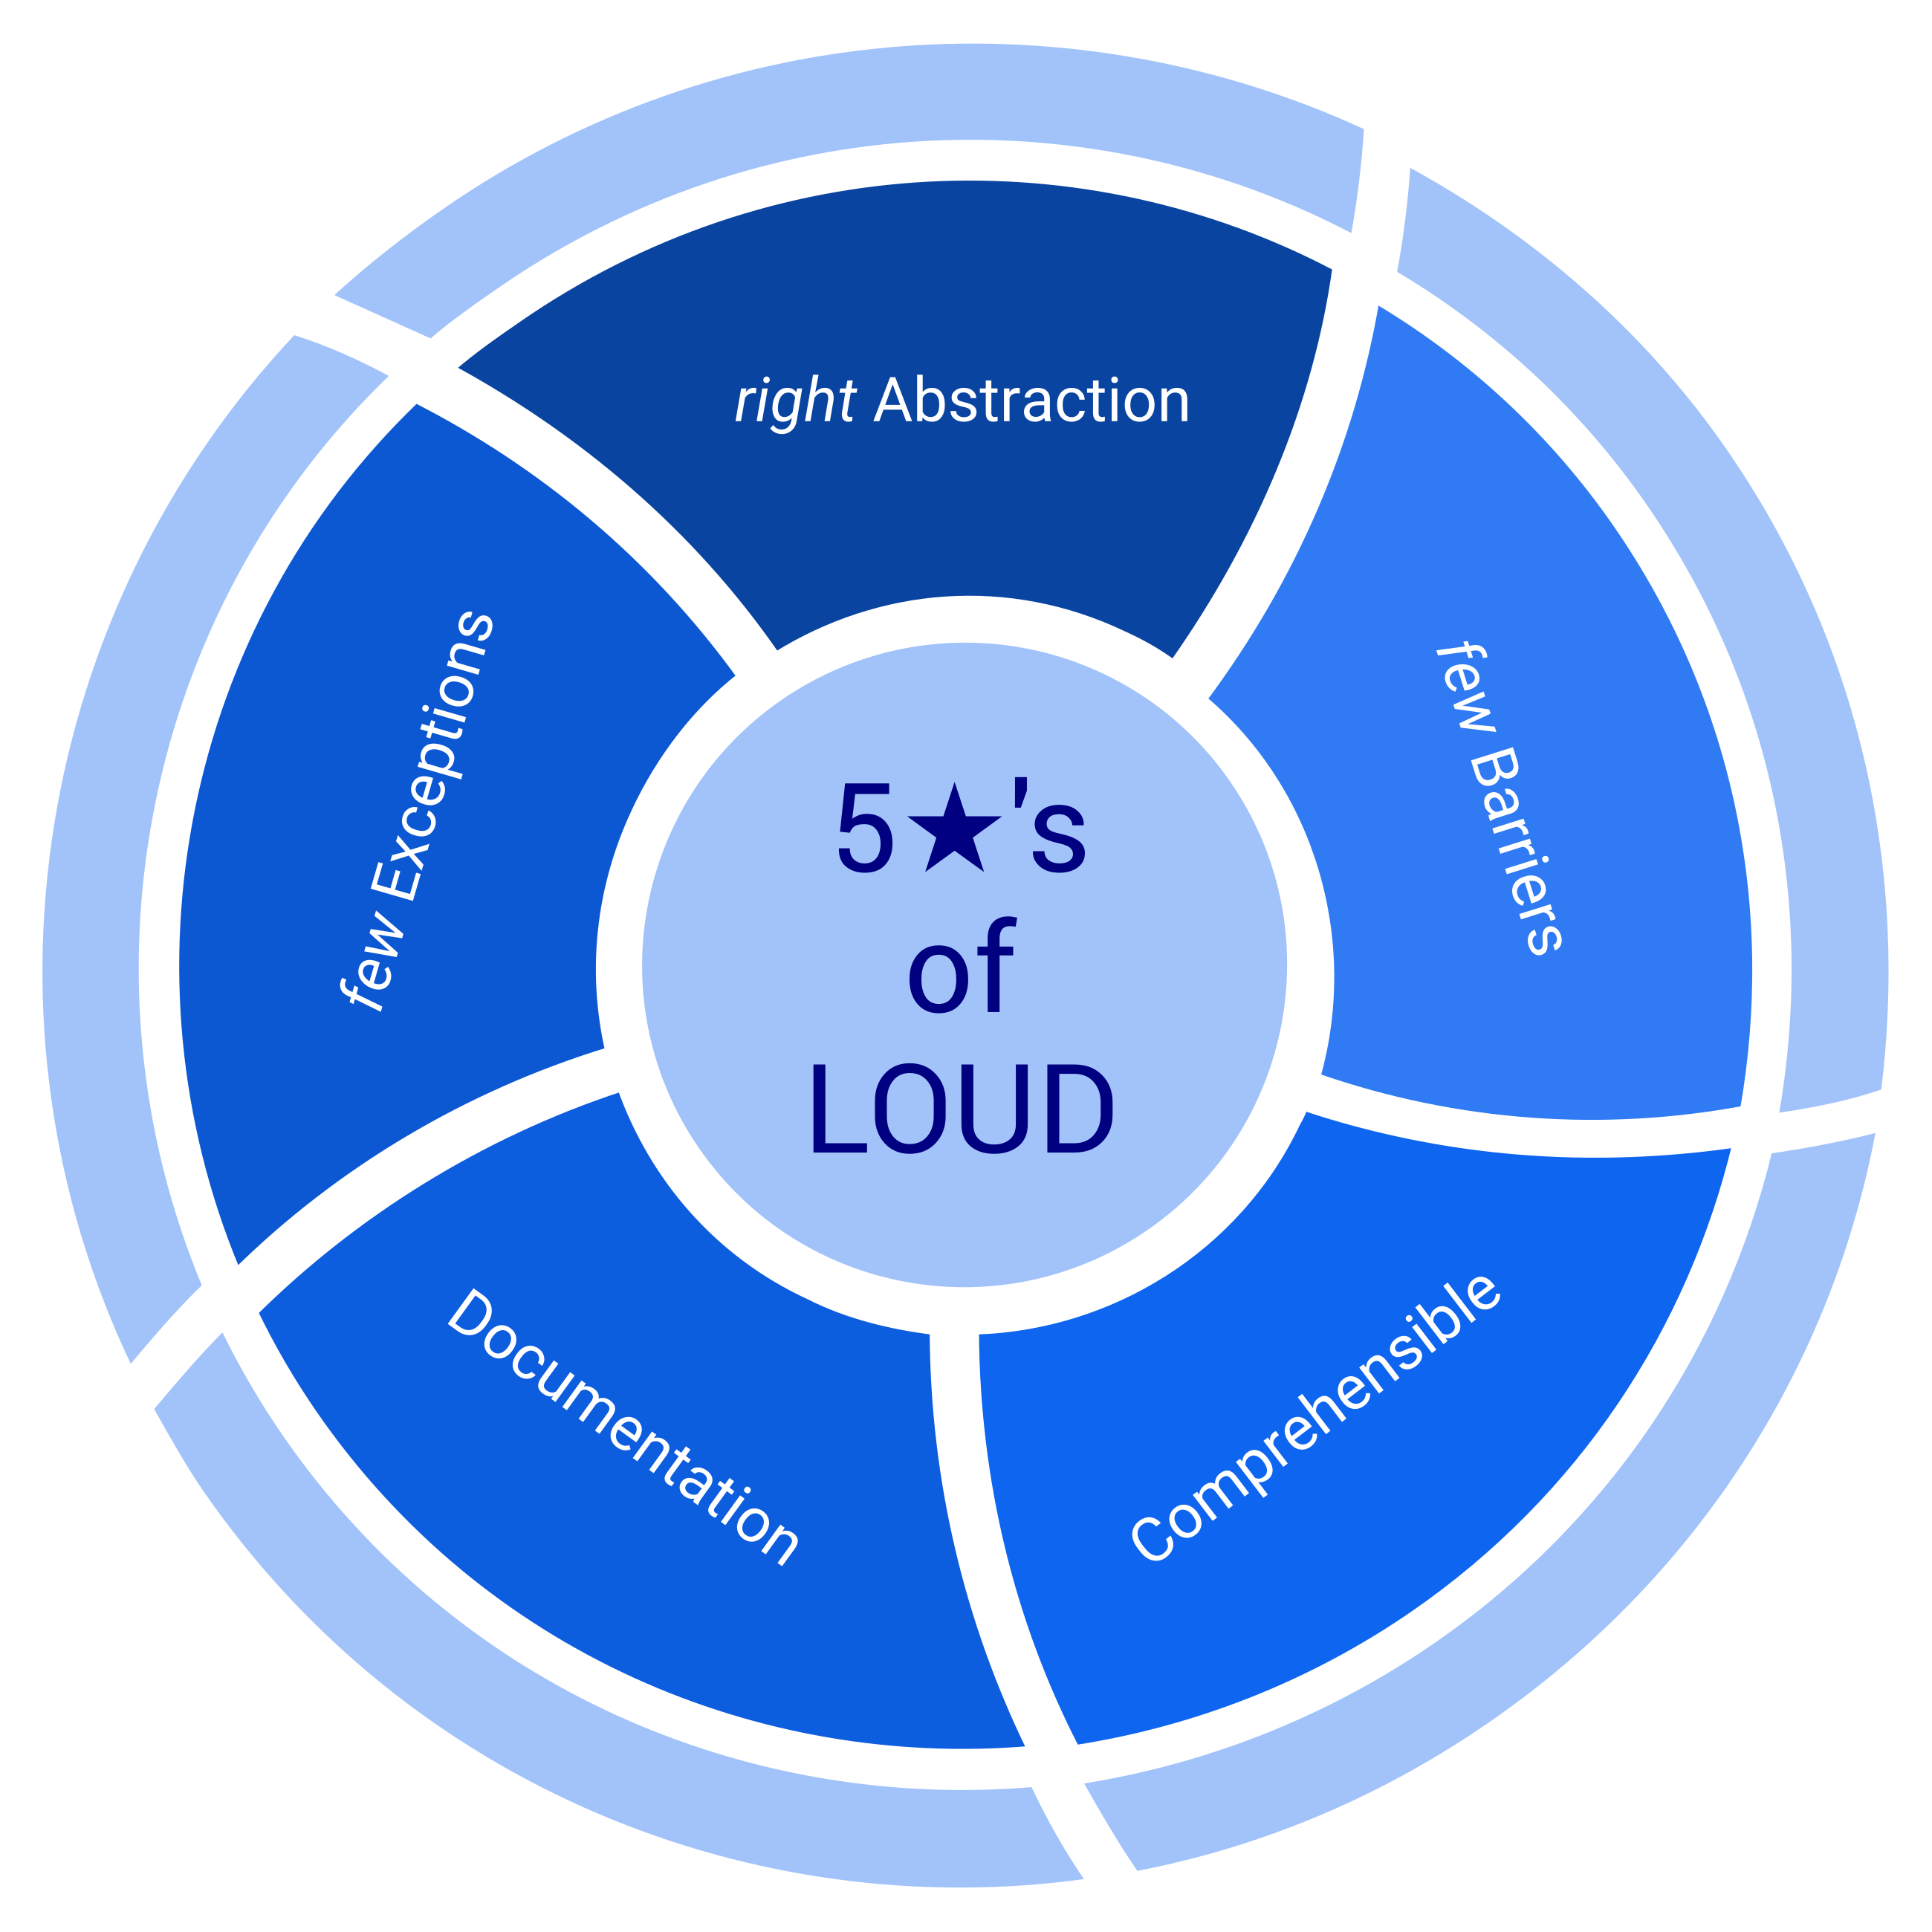
\includegraphics[width=8cm]{5_Star_LOUD.png}
\caption{5 Star LOD, Florian Thiery [CC BY 4.0]}
\label{loud}
\end{center}
\end{figure}

\section{FAIR data}

LOUD data are not enough. In 2014 at the Lorentz workshop \footnote{\url{https://www.force11.org/group/fairgroup/fairprinciples}} the term \textit{FAIR} (Fig.~\ref{fair}) [Findable, Accessible, Interoperable, Reusable] was launched and the resulting 15 FAIR principles were published\cite{wilkinson_fair_2016} in 2016 \cite{force11_fair_2016}.

\begin{figure}[!htb]
\begin{center}
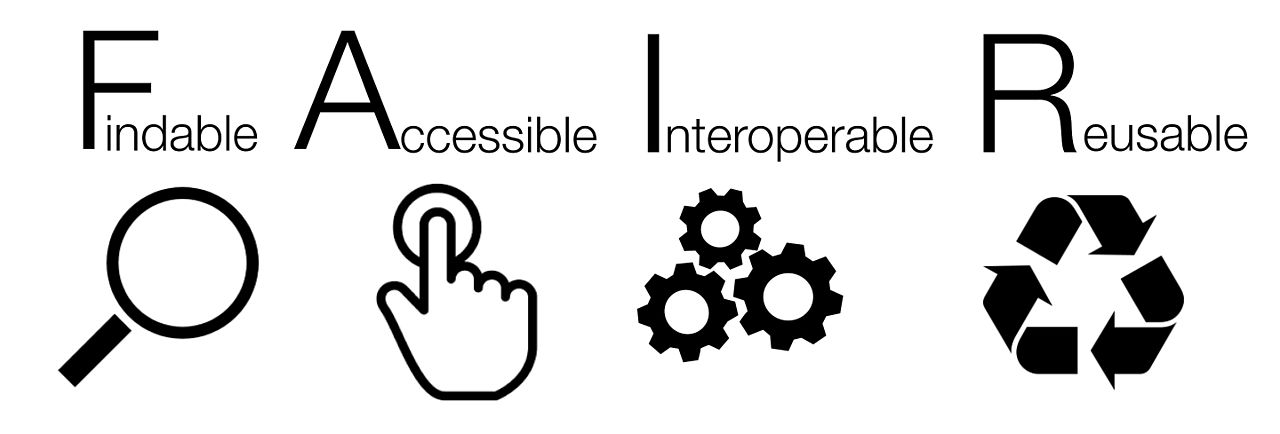
\includegraphics[width=8cm]{FAIR_data_principles.jpg}
\caption{FAIR data principles, SangyaPundir [CC BY-SA 4.0]}
\label{fair}
\end{center}
\end{figure}

The FAIR Guiding Principles are\cite{wilkinson_fair_2016}:

To be Findable

\textit{F1. (meta)data are assigned a globally unique and persistent identifier}

\textit{F2. data are described with rich metadata (defined by R1 below)}

\textit{F3. metadata clearly and explicitly include the identifier of the data it describes}

\textit{F4. (meta)data are registered or indexed in a searchable resource}

To be Accessible

\textit{A1. (meta)data are retrievable by their identifier using a standardized communications protocol}

\textit{A1.1 the protocol is open, free, and universally implementable}

\textit{A1.2 the protocol allows for an authentication and authorization procedure, where necessary}

\textit{A2. metadata are accessible, even when the data are no longer available}

To be Interoperable

\textit{I1. (meta)data use a formal, accessible, shared, and broadly applicable language for knowledge representation.}

\textit{I2. (meta)data use vocabularies that follow FAIR principles}

\textit{I3. (meta)data include qualified references to other (meta)data}

To be Reusable

\textit{R1. meta(data) are richly described with a plurality of accurate and relevant attributes}

\textit{R1.1. (meta)data are released with a clear and accessible data usage license}

\textit{R1.2. (meta)data are associated with detailed provenance}

\textit{R1.3. (meta)data meet domain-relevant community standards}

\section{Sphere 7 Data}

Merging all the mentioned principals above, reaching not only LOD, not LOUD, not FAIR but LOUD and FAIR research data, we need a new stairway to the Olympus of semantic data modelling. Therefore we can have a look into history and Aristotle’s idea of seven spheres of heaven, see Fig.~\ref{sphere}.

\begin{figure}[!htb]
\begin{center}
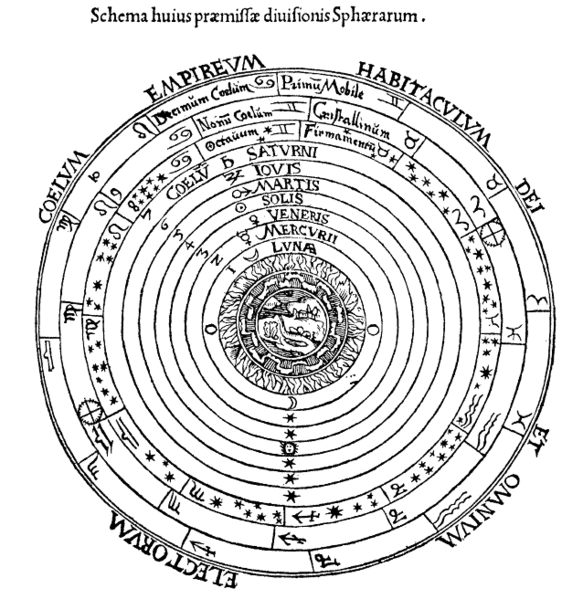
\includegraphics[width=8cm]{583px-Ptolemaicsystem-small.png}
\caption{Ptolemaic System, Fastfission [Public domain]}
\label{sphere}
\end{center}
\end{figure}

This model in mind, I propose the \textcolor[rgb]{0.5,0,0.5}{\textbf{Sphere 7 Data Model}}, or \textcolor[rgb]{0.5,0,0.5}{\textbf{Model of Seven Data Spheres}}, as displayed in Fig.~\ref{ssd}. This sphere model combines all the mentions principles to reach the seventh sphere of heaven via LOUD FAIR research data.

\begin{figure}[!htb]
\begin{center}
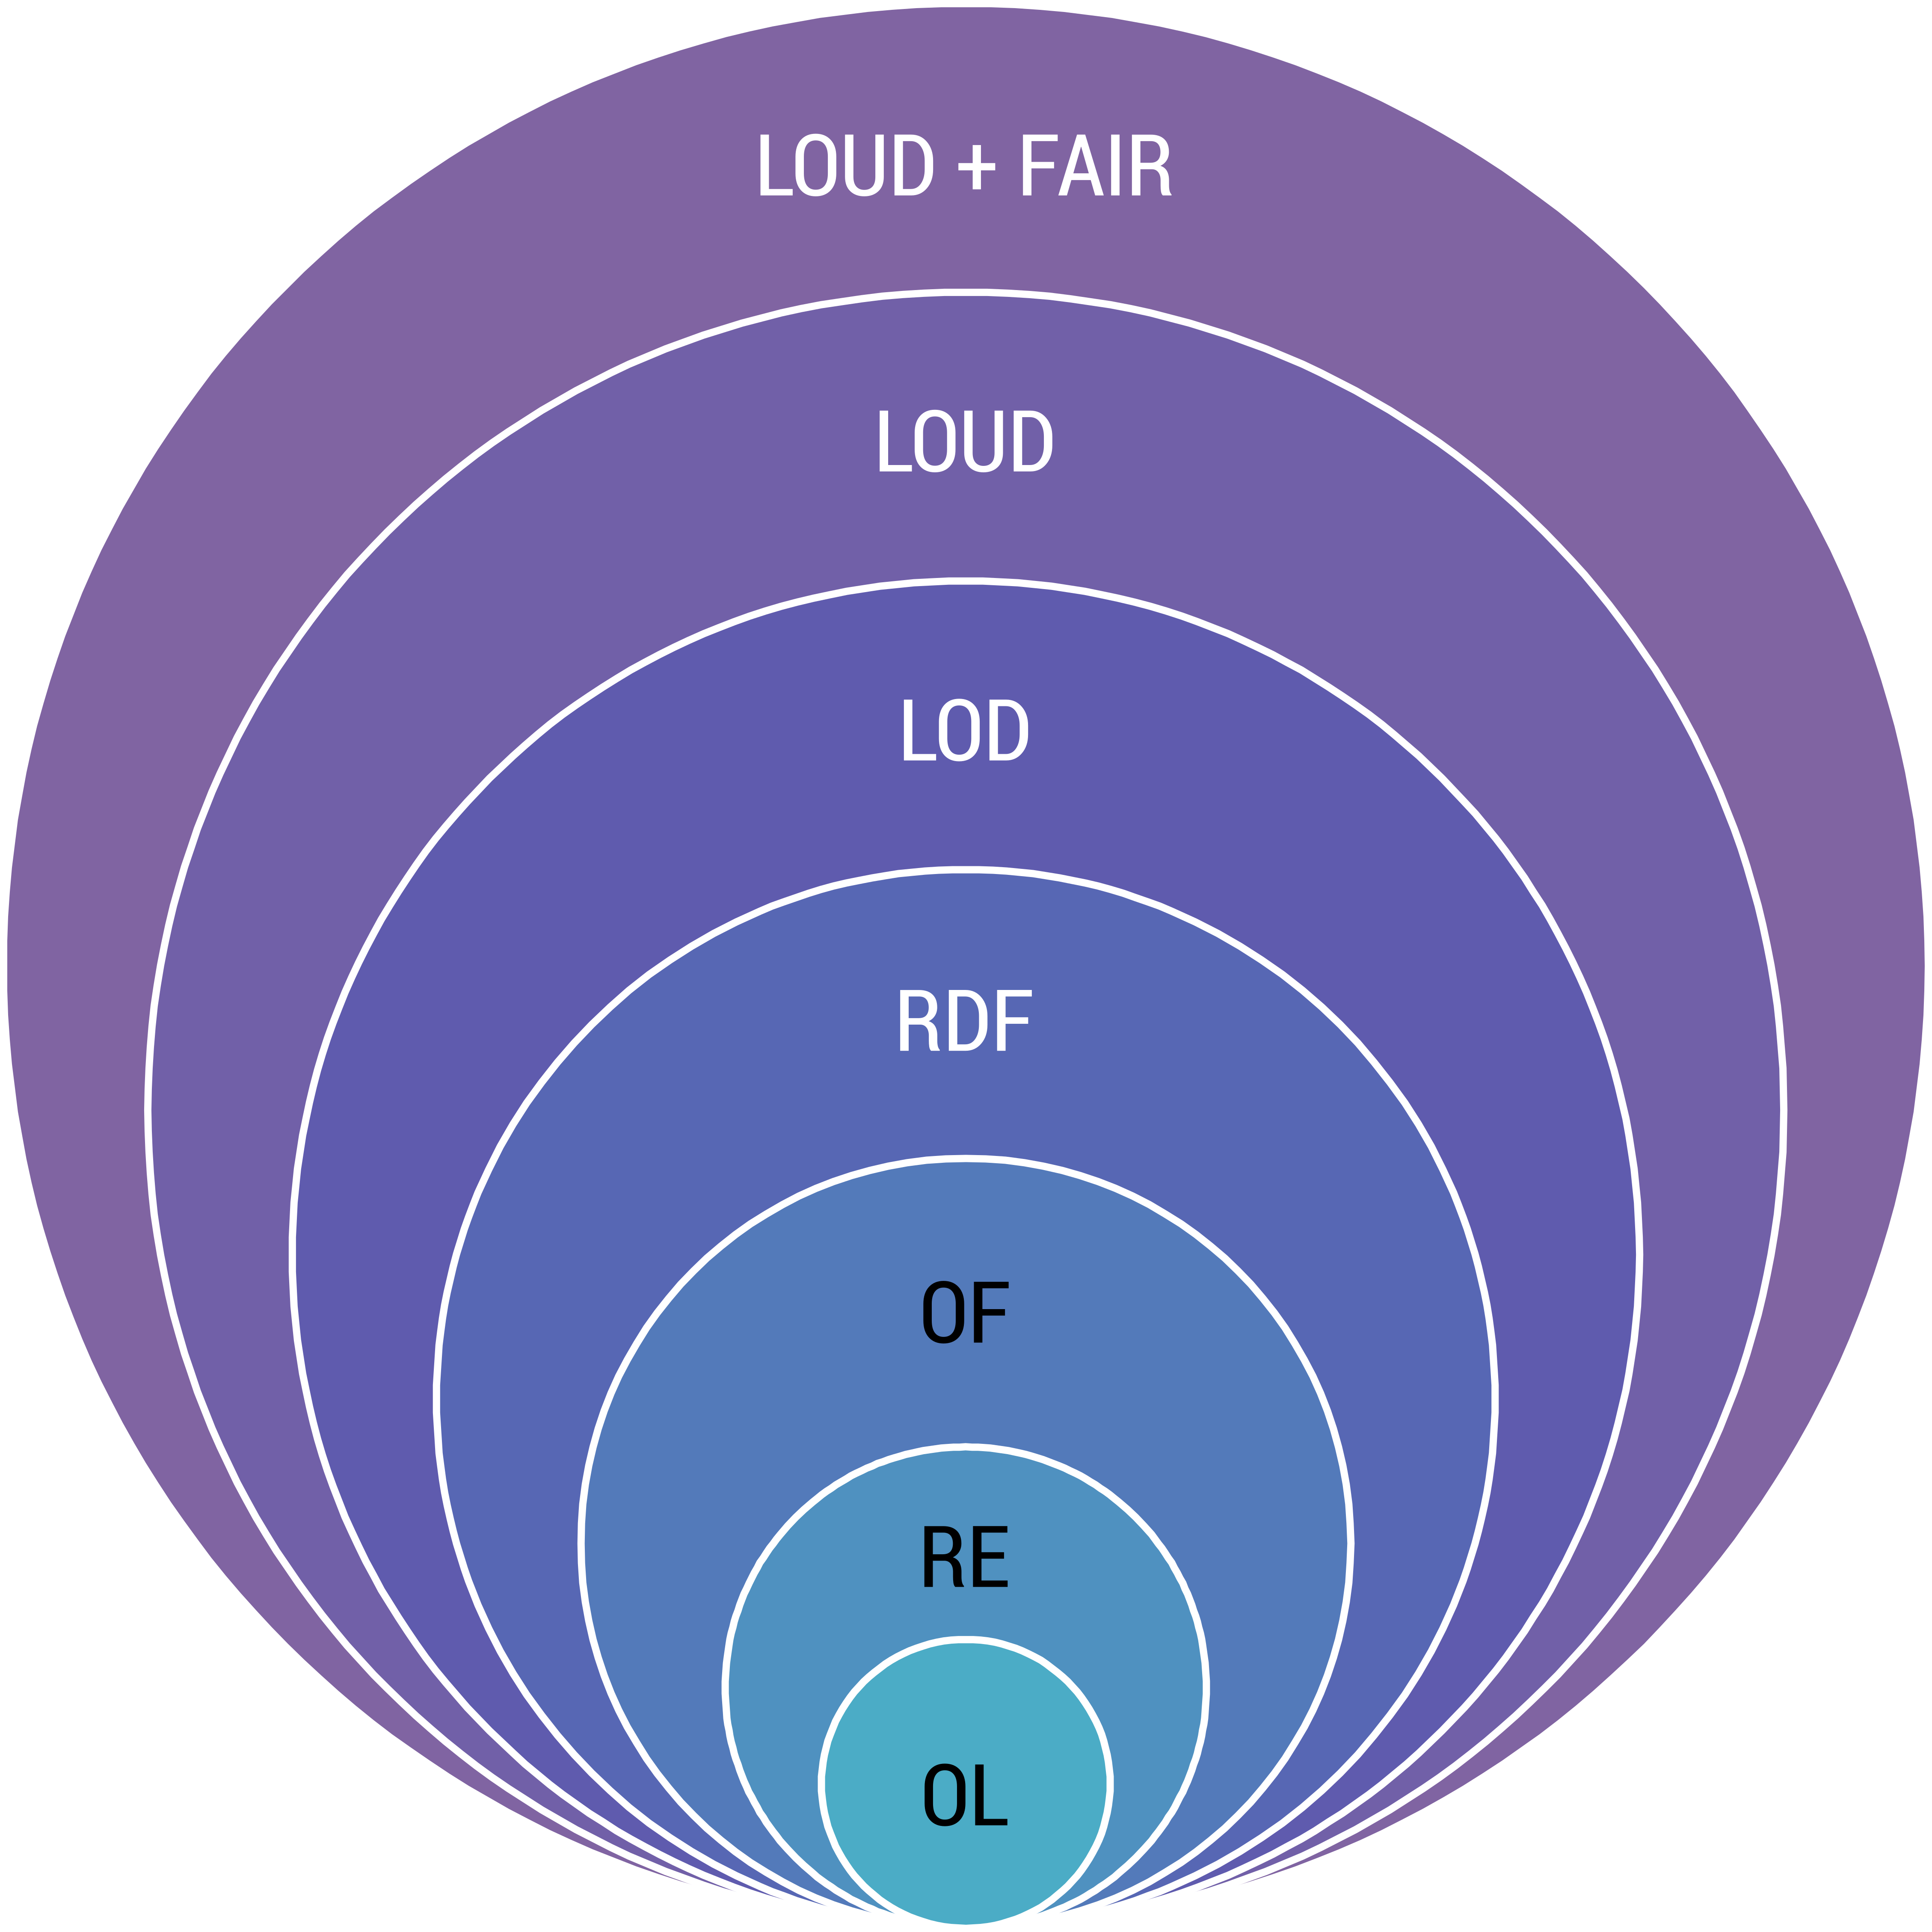
\includegraphics[width=8cm]{Loud_fair_sphere.png}
\caption{Seven Sphere Data, Florian Thiery [CC BY 4.0]}
\label{ssd}
\end{center}
\end{figure}

The \textbf{\textcolor[rgb]{0.5,0,0.5}{single spheres}} are defined as follows:

\textcolor[rgb]{0.5,0,0.5}{\textbf{1. Sphere: OL}}

Data is available in the Web under a open license.

\textcolor[rgb]{0.5,0,0.5}{\textbf{2. Sphere: RE}}

Data is available as structured machine readable data.

\textcolor[rgb]{0.5,0,0.5}{\textbf{3. Sphere: OF}}

Data is available in an open, non-proprietary, structured machine readable data format.

\textcolor[rgb]{0.5,0,0.5}{\textbf{4. Sphere: RDF}}

Data is available as URIs and semantically modelled as RDF.

\textcolor[rgb]{0.5,0,0.5}{\textbf{5. Sphere: LOD}}

Data is available as resource, semantically modelled as RDF and semantically linked to other resources.

\textcolor[rgb]{0.5,0,0.5}{\textbf{6. Sphere: LOUD}}

LOD is available as usable data, according to the LOUD principles.

\textcolor[rgb]{0.5,0,0.5}{\textbf{7. Sphere: LOUD + FAIR}}

LOUD is available as findable, accessible, interoperable and reusable data, according to the FAIR principles.

\begin{ack}                               
I would like to thank the Mainz Centre for Digitality in the Humanities and Cultural Studies (mainzed) and R\"omisch-Germanisches Zentralmuseum for supporting me.
\end{ack}

\bibliographystyle{IEEEtran}
\bibliography{autosam}

\end{document}